% Chapter Template
\chapter{Discussion of survey results}
\label{chapter4}

In total, 31 responses were collected. The majority of respondents majored in law (58\%) vs non-law (42\%) respondents (Figure~\ref{fig:demo_1}). Except for the questions relating to subject matter expertise (data privacy and AI), the level of agreement of law vs non-law respondents about their beliefs relating to data privacy and AI were about the same (Figure~\ref{fig:demo_3}). Law respondents had less expertise in AI, while conversely, non-law respondents had less experience with data privacy. Across all respondents, while they rated that decisions by AI could be a risk to society (about 4), they also agreed that decisions by AI could be equally useful. This perhaps suggests that the respondents think the balance between "usefulness" and "risks" are not zero-sum; AI could be very helpful in solving problems, but at the same time users should be cognisant of the risks.

I mainly used sentences annotated as \texttt{Identifier Cookie 1st Party} to produce explanations for the survey. This is because the class performance of \texttt{Identifier Cookie 1st Party} performed relatively well, and has the highest number of instances in the dataset which provides a large variety of drafting styles.

\begin{figure}[!ht]
  \centering
  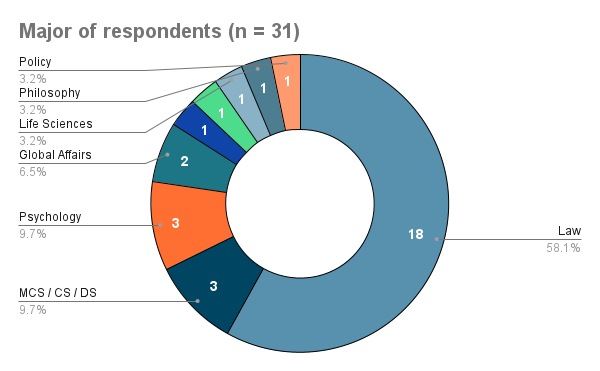
\includegraphics[width=0.85\linewidth]{figures/major_respondents.png}
  \caption{Breakdown of respondents' expertise by major}
  \label{fig:demo_1}
\end{figure}

% \begin{table}[!ht]
%     \resizebox{\textwidth}{!}{
%     \begin{tabular}{|p{0.45\linewidth}|l|l|}
%     \hline
%     \textbf{Major / Expected major}                    & \textbf{Count} & \textbf{Percentage of total (\%)} \\ \hline
%     Law                                                & 18             & 58                                \\ \hline
%     MCS / Computer Science / Data Science / Statistics & 3              & 9.7                               \\ \hline
%     Psychology                                         & 3              & 9.7                               \\ \hline
%     Global Affairs / Political Science                 & 2              & 6.5                               \\ \hline
%     Environmental Studies                              & 1              & 3.2                               \\ \hline
%     Economics                                          & 1              & 3.2                               \\ \hline
%     Life Sciences                                      & 1              & 3.2                               \\ \hline
%     Philosophy                                         & 1              & 3.2                               \\ \hline
%     Policy                                             & 1              & 3.2                               \\ \hline
%     \end{tabular}
%     }
%     \caption{Demographic breakdown of respondents according to academic discipline}
%     \label{tab:demo_1}
% \end{table}

\begin{figure}[!ht]
    \begin{subfigure}[b]{1\textwidth}
      \centering
      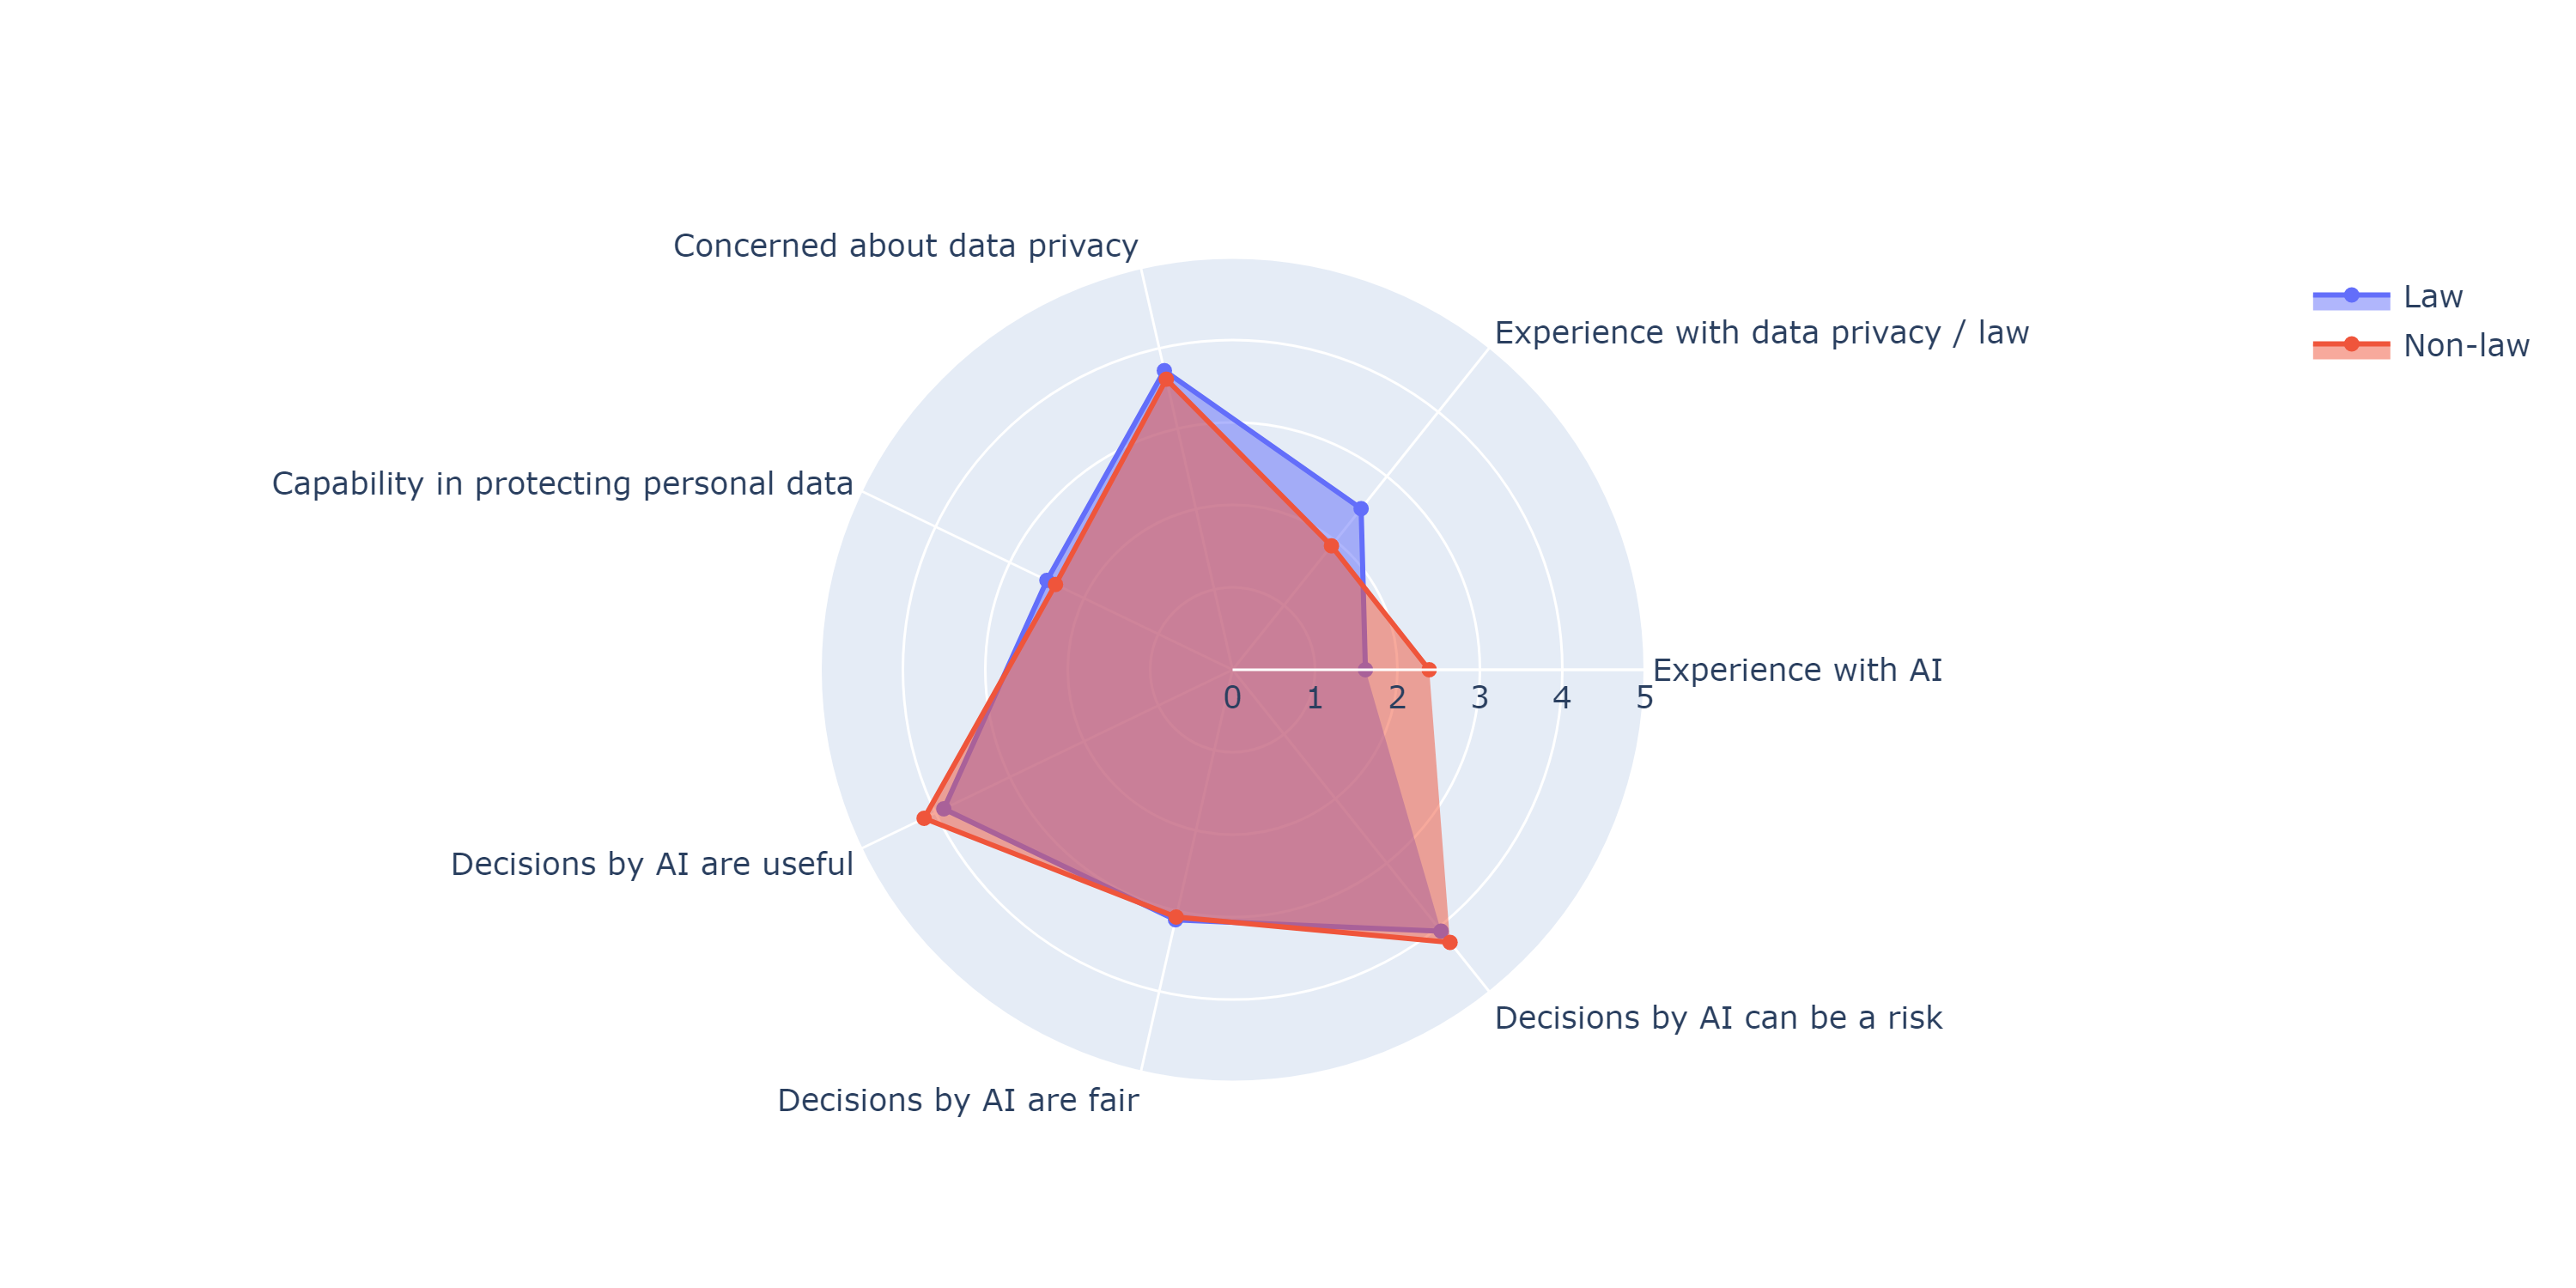
\includegraphics[width=1\linewidth]{figures/demo_3.png}
      \caption{Law vs Non-law respondents}
    \end{subfigure}
    \hfill
    \begin{subfigure}[b]{1\textwidth}
      \centering
      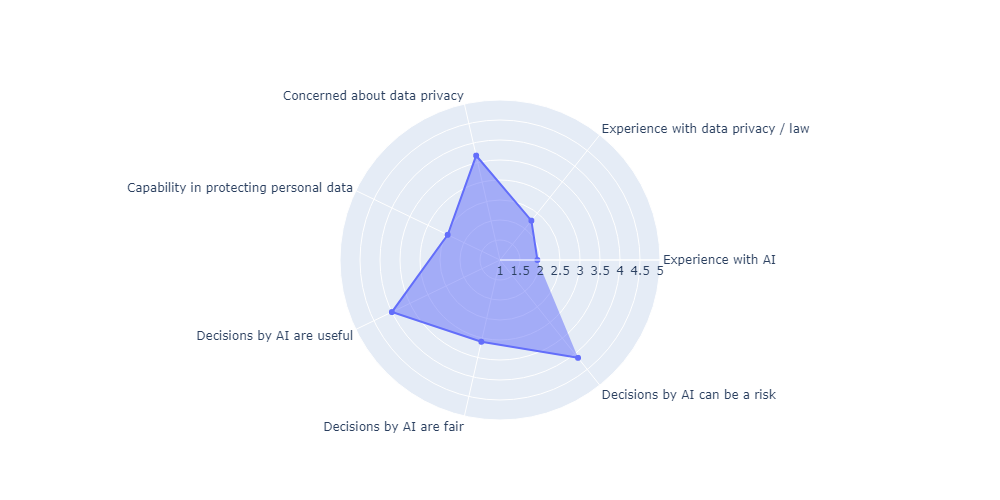
\includegraphics[width=1\linewidth]{figures/demo_4.png}
      \caption{All respondents}
    \end{subfigure}
    \caption{Mean scores of self-reported beliefs of respondents regarding AI \& data privacy. (1 = least agree, 5 = strongly agree. $n=31$)}
    \label{fig:demo_3}
\end{figure}

\section{Part 2 \& Part 6: Comparison of self-reported scores of explainability across the three contexts}
\label{sec:three_contexts_comparison}
Using the Wilcoxon Rank Sum Test as the distribution of the scores are likely nonparametric, I tested for the following, setting $\alpha = 0.1$: 

\noindent H0: There is no increase / decrease in scores after viewing the explainations.

\noindent H1: There is an increase / decrease in scores after viewing the explainations.

The 1-sided test was used to check whether the distribution underlying the difference between the initial and final paired scores was symmetric below or above 0 \cite{scipy}. Mathematically this difference can be stated as $d = i - f$, where $i$ and $f$ are the scores reported before and after viewing the explanations, and $d$ is the difference. Hence, if $d < 0$, then $i < f$ and the scores increased after viewing. Conversely, if $d > 0$, then $i > f$ and the scores decreased after viewing. p-values are reported in Table~\ref{tab:context_comparison} and~\ref{tab:context_comparison_2}. For Table~\ref{tab:context_comparison_2a} and~\ref{tab:context_comparison_2b}, I took the mean of self-reported scores across metrics, and across contexts respectively. For Table~\ref{tab:context_comparison_2c}, the self-reported scores were averaged across both context and metric. The trending in scores for each metric across the contexts are visualised in Figure~\ref{fig:part2_part6_comparison}.

\begin{table}[!ht]
    \centering
    \resizebox{\textwidth}{!}{    
    \begin{tabular}{|p{0.3\textwidth}|p{0.15\textwidth}|p{0.15\textwidth}|p{0.15\textwidth}|p{0.15\textwidth}|p{0.15\textwidth}|p{0.15\textwidth}|}
    \hline
        \textbf{Question} & \textbf{Context 1: Increase} & \textbf{Context 1: Decrease} & \textbf{Context 2: Increase} & \textbf{Context 2: Decrease} & \textbf{Context 3: Increase} & \textbf{Context 3: Decrease} \\ \hline
        \textbf{Do you think model is effective?} & \cellcolor{red!25}0.013 & 0.987 & 0.932 & \cellcolor{red!25}0.0684 & 0.856 & 0.144 \\ \hline
        \textbf{Do you think model is a fair method?} & 0.382 & 0.618 & 0.841 & 0.159 & 0.933 & \cellcolor{red!25}0.0671 \\ \hline
        \textbf{Do you think model is a risk to society?} & 0.756 & 0.244 & 0.428 & 0.572 & 0.825 & 0.175 \\ \hline
        \textbf{Do you trust the prediction of the model?} & 0.887 & 0.113 & 0.945 & \cellcolor{red!25}0.055 & 0.837 & 0.163 \\ \hline
    \end{tabular}
    }
    \caption{p-values comparing whether there was a statistically significant increase / decrease in the explainability scores before and after viewing explanations.}
    \label{tab:context_comparison}
\end{table}

\begin{table}[!ht]
    \centering
    \begin{subtable}[h]{0.45\textwidth}
      \centering  
      \begin{tabular}{|l|l|}
        \hline
            \textbf{Context} & \textbf{p-value} \\ \hline
            1: Increase & 0.369 \\ \hline
            1: Decrease & 0.633 \\ \hline
            2: Increase & 0.940 \\ \hline
            2: Decrease & \cellcolor{red!25}0.060 \\ \hline
            3: Increase & 0.955 \\ \hline
            3: Decrease & \cellcolor{red!25}0.0450 \\ \hline
        \end{tabular}
        \caption{p-values by context, taking the mean of scores across metrics}
        \label{tab:context_comparison_2a}
    \end{subtable}
    \hfill
    \begin{subtable}[h]{0.45\textwidth}
      \centering  
      \begin{tabular}{|l|l|}
            \hline  
            \textbf{Metric}                                    & \textbf{p-value}                     \\ 
            \hline
            Effective: Increase & 0.485  \\ \hline
            Effective: Decrease & 0.515  \\ \hline
            Fair: Increase      & 0.826  \\ \hline
            Fair: Decrease      & 0.174  \\ \hline
            Risk: Increase      & 0.660  \\ \hline
            Risk : Decrease     & 0.340  \\ \hline
            Trust: Increase     & 0.953  \\ \hline
            Trust: Decrease     & \cellcolor{red!25}0.0468 \\ \hline
        \end{tabular}
        \caption{p-values by metric, taking the mean of scores across contexts}
        \label{tab:context_comparison_2b}
    \end{subtable}
    \hfill
    \begin{subtable}[h]{0.45\textwidth}
      \centering
      \begin{tabular}{|l|l|}
        \hline
        \textbf{Increase} & \textbf{Decrease} \\ \hline
        0.844             & 0.156           \\ \hline
      \end{tabular}
    \caption{p-values taking the mean scores across contexts and metrics}
    \label{tab:context_comparison_2c}
    \end{subtable}
    \caption{p-values comparing mean scores (cells highlighted in red are statistically significant)}
    \label{tab:context_comparison_2}
\end{table}

\begin{figure}[!ht]
  \centering
  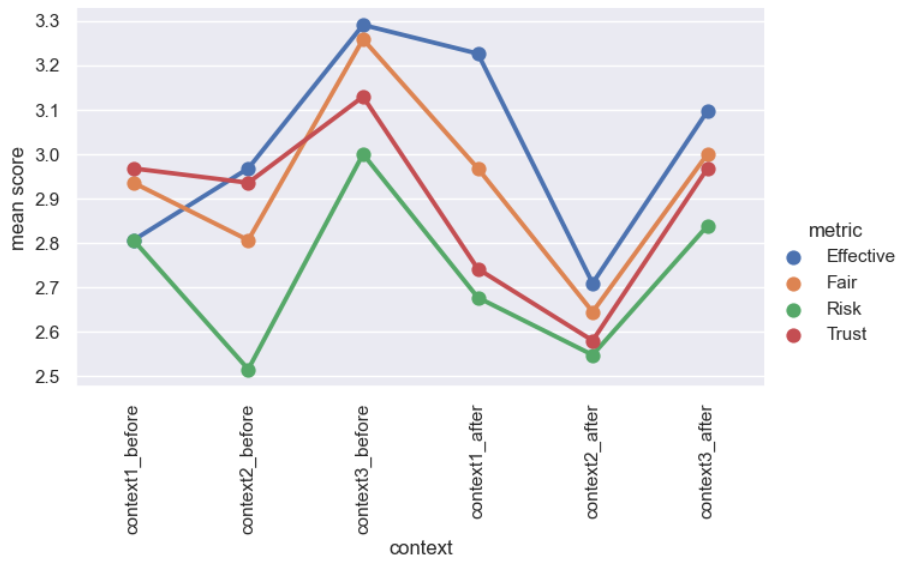
\includegraphics[width=1\linewidth]{figures/part2_part6_metric_comparison.png}
  \caption{Mean scores for each metric and each context before and after respondents viewed explanations}
  \label{fig:part2_part6_comparison}
\end{figure}


Here are the instances when $p<0.1$, and therefore $H0$ can be rejected in favour of $H1$:
\begin{enumerate}
    \item Effectiveness and trust significantly decreased for context 2 (PDPC), and fairness significantly decreased for context 3 (user). Effectiveness significantly increased for context 1 (app developer) (Table~\ref{tab:context_comparison}).
    \item There is a statistically significant decrease in explainability metrics for context 1 and 2 when taking the mean of the scores across the metrics (Table~\ref{tab:context_comparison_2a}) and for trust across the three contexts (Table~\ref{tab:context_comparison_2b}). 
    \item Interestingly, there seems to be a higher correlation between the scores of the 4 metrics specifically for context 2 and 3 after the respondents viewed the explanations (Figure~\ref{fig:part2_part6_comparison}).
\end{enumerate}

The explanations presented to respondents were deliberately chosen to demonstrate the limitations of the model (see Figure~\ref{fig:part4_explanations}). Hence, respondents were likely more cognisant of such limitations\footnote{This can also be inferred from the negative trend of interpretability and understandability as explained \hyperref[sec:interpret_understand]{below}.} when they answered the same questions again in Part 6. Here are some inferences that I draw from these observations:
\begin{enumerate}
    \item \textit{"Efficiency" is dependent on the risks of making wrong predictions (App developer, PDPC)}: The speed of automation of reading privacy policies would be the same regardless whether an app developer or PDPC uses it. However, changes in efficiency differed between the two contexts, suggesting that automation was not the only metric that respondents considered part of "effectiveness". Respondents could have considered that automation was more important to app developers when balanced against the risks of making a wrong prediction, as compared to the PDPC, where the risks were too high to justify automation. Hence, the classifier is not "effective" in terms of making a legally defensible decision given that it is fallible.
    
    \item \textit{Classifier's interpretability is especially critical for the PDPC such that trust was affected}: Respondents could have thought that PDPC, as a regulatory body in comparison to app developers and users who are not, should fully understand and explicitly justify the decision of finding an organisation (such as an app developer) liable for breaching the PDPA. Hence, when respondents reported a drop in overall interpretability and understandability, it especially affected their trust in the logic of the classifier.
    
    \item \textit{Fairness is perceived in relation to the user's own interests, rather than systemic fairness}: If respondents believed that the logic of the classifier was unfair because it would unfairly discriminate against a certain style of writing data privacy policies (a kind of "systemic fairness"), respondents would also have reported a drop in fairness for the PDPC context as there would be the most expectation on a regulatory body to treat data subjects and organisations fairly. However, fairness only dropped for the user and not the PDPC. Respondents may have defined fairness as the inability to get recourse for violated data rights due to wrong classifier predictions affecting their legal claims. In this way, respondents were only concerned with their own interests.
     
    \item \textit{Expertise of the end user of explanations affects explainability metrics}: In relation to the overall drop in explainability metrics for the contexts of the PDPC and the user, perhaps the respondents thought that PDPC and the user did not have technical knowledge to better understand the classifier's logic beyond the explanations that were presented to them, whereas the app developer would have such technical knowledge. Hence, the lack of technical expertise of the PDPC and the user caused the drop in explainability metrics.
     
    \item \textit{Mismatch in expectations particularly affects trust}: In the case of trust being the only metric that significantly decreased across the contexts, this could point to a mismatch of expectations. Intuitively, if respondents do not understand how a process works, they are less likely to trust the results of that process. Perhaps respondents' expectations of AI was that AI would reason similarly to how humans would, or that AI functioned entirely objectively similar to applying a formula in Excel where it is clear how the result was obtained from the formula. Instead, the explanations provided showed that the classifier was inconsistent, sometimes relying heavily on words like "cookies" and other times not so much without any discernible reason. So respondents' expectations were not met, and this caused the overall drop in trust.
\end{enumerate}

Notably, trust was the only value that decreased overall. The intuition behind increasing explainability is to increase trust of users. Trust is especially important to the judicial process as it is closely related to confidence and compliance with court decisions \cite{goodman2021}. Hence, this relationship between explainability and trust is worth further investigation because there is evidence that shows this relation is not as general as previously thought \cite{kastner2021}. In fact, if explanations reveal problems about the system, trust could decrease rather than increase. This could be a possible explanation of the results because respondents were intentionally given examples that demonstrated the limitations of the classifiers.

One strand of analysis that was not borne by the results is the relation between the consequences of a wrong decision and the level of explainability required. Intuitively, even if an e-commerce AI recommendation algorithm were to recommend a product to a consumer which did not meet their preferences, it would pose little consequence other than (perhaps) mild irritation. In comparison, if an algorithmic judge convicted the wrong person for murder, it would have irreversible consequences. Hence in the latter scenario, the algorithmic decision-making must be highly transparent. In fact, the AI Act proposed by the European Commission has relied on this relation. It differentiates AI systems into those which are "high risk" and "medium risk", with "high risk" systems requiring a greater level of explainability that is user-empowering and compliance-oriented \cite{sovrano2022metrics}.

However, the respondents' reported scores of risk for all the contexts did not significantly change after viewing the explanations. As previously \hyperref[sec:survey_method]{mentioned}, I intentionally made sure that the legal consequences of making a wrong decision was capped monetarily at \$10,000 for all contexts because I wanted to reduce the amount of legal knowledge necessary to understand the contexts. However, I did not specifically restrict respondents from assuming that there could be other non-legal consequences. Nevertheless, perhaps the lack of significant result was due to the phrasing of the question that was posed to respondents as "risk to society" which could be interpreted to be a much broader claim rather than just "risk".

\section{Part 3: Testing whether viewing more visualisations affected explainability}
\subsection{Analysis of reported interpretability and understandability}
\label{sec:interpret_understand}
There is a decreasing trend of both understandability and interpretability after viewing each explanation (Figure~\ref{fig:part3_trend}, explanations can be viewed in Figure~\ref{fig:part4_explanations}). Using the Wilcoxon Rank Sum Test, I separately tested for significant differences of understandability and interpretability, setting $\alpha = 0.1$: 

\noindent H0: There is no difference in reported interpretability / understandability between the first and last questions.

\noindent H1: There is an increase / decrease of reported interpretability / understandability between the first and last questions.

\begin{table}[!ht]
  \centering
  \begin{tabular}{l|l|l|}
  \cline{2-3}
                                                & \textbf{Increase} & \textbf{Decrease} \\ \hline
  \multicolumn{1}{|l|}{\textbf{Interpretable}} & 0.867             & 0.132             \\ \hline
  \multicolumn{1}{|l|}{\textbf{Understandable}}  & 0.999             & \cellcolor{red!25}\textless{}0.001  \\ \hline
  \end{tabular}
  \caption{p-values comparing reported understandability and interpretability between the first and last question (cells highlighted in red are statistically significant)}
  \label{tab:p_values_interpret_understand}
\end{table}

\begin{figure}[!ht]
  \centering
  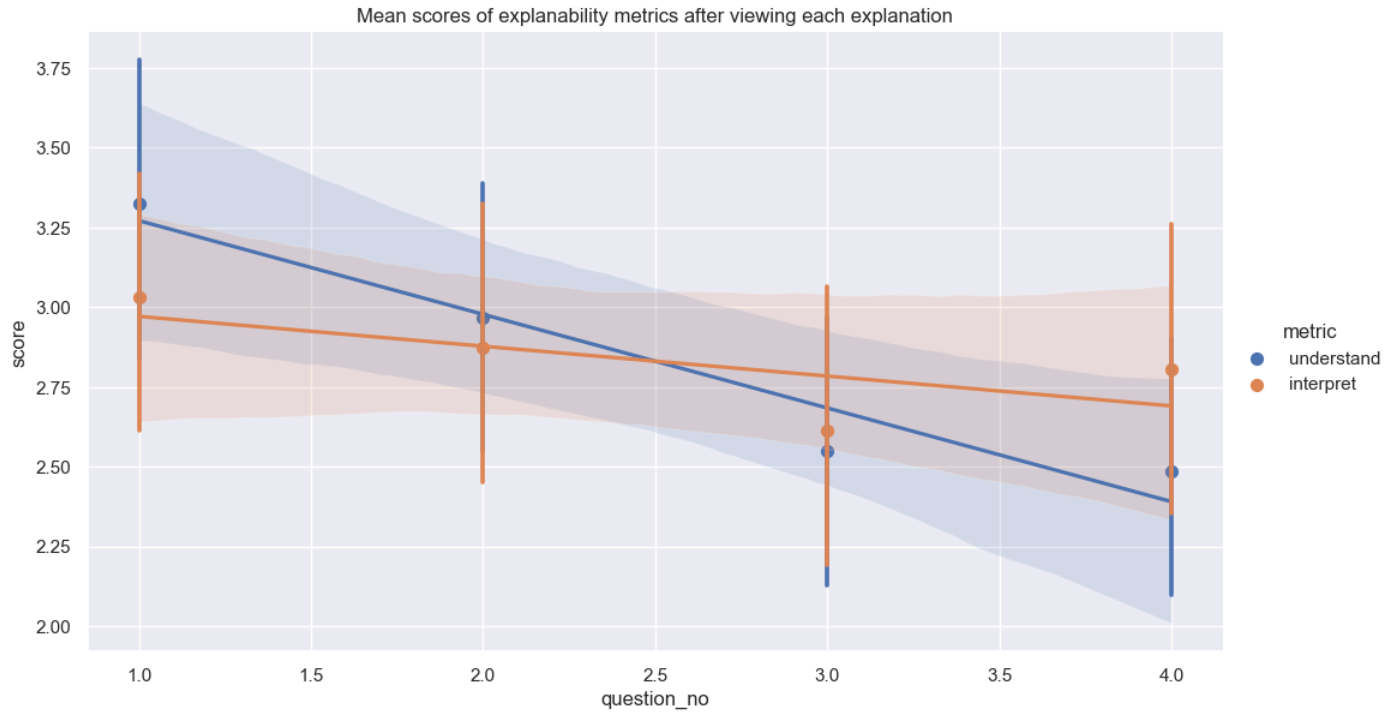
\includegraphics[width=1\linewidth]{figures/part3.png}
  \caption{Trend of the mean of self-reported understanding and interpretability after viewing each explanation}
  \label{fig:part3_trend}
\end{figure}

\begin{figure}[!ht]
  \begin{subfigure}[b]{1\textwidth}
    \centering
    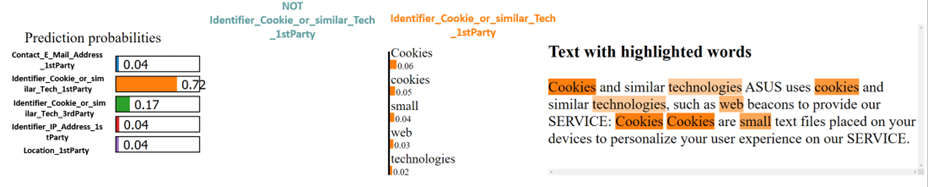
\includegraphics[width=1\linewidth]{figures/explanations_visualisations/section_4a/Picture1.png}
    \caption{1}
  \end{subfigure}
  \hfill
  \begin{subfigure}[b]{1\textwidth}
    \centering
    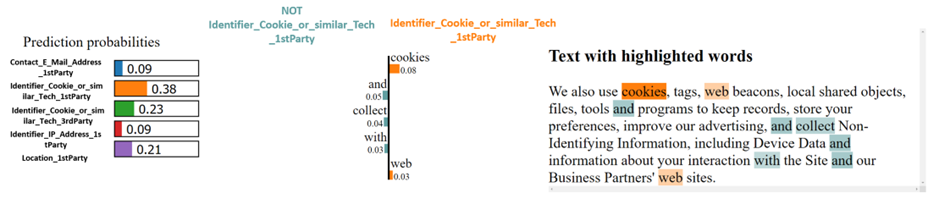
\includegraphics[width=1\linewidth]{figures/explanations_visualisations/section_4a/Picture2.png}
    \caption{2}
  \end{subfigure}
  \hfill
  \begin{subfigure}[b]{1\textwidth}
    \centering
    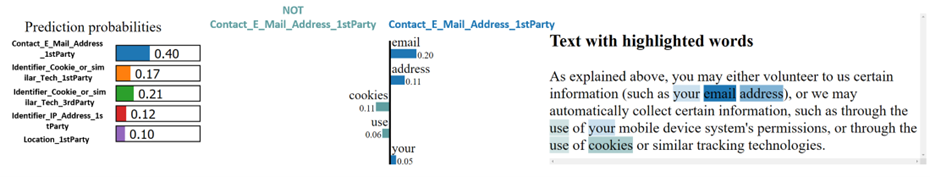
\includegraphics[width=1\linewidth]{figures/explanations_visualisations/section_4a/Picture3.png}
    \caption{3}
  \end{subfigure}
  \hfill
  \begin{subfigure}[b]{1\textwidth}
    \centering
    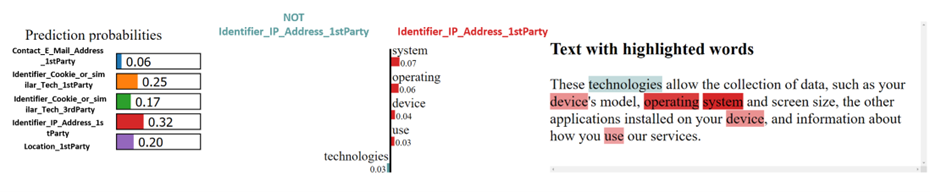
\includegraphics[width=1\linewidth]{figures/explanations_visualisations/section_4a/Picture4.png}
    \caption{4}
  \end{subfigure}
  \caption{The 4 visualisations shown to respondents. Respondents were asked to rate how far they understood why the model made the prediction, and how far they found the visualisation easy to interpret. All 4 sentences were annotated as \texttt{Identifier Cookie 1st Party}.}
  \label{fig:part4_explanations}
\end{figure}

There was a statistically significant decrease in understandability but not interpretability (Table~\ref{tab:p_values_interpret_understand}). Hence, H0 can be rejected in favour of H1. 

A reason for why there was no significant decrease in interpretability was because the questions I posed to the respondents were clear in distinguishing the visualisation from the classifier's logic\footnote{The two questions posed to respondents were: (1) Do you understand why the model made the prediction? and (2) Did you find the visualisation easy to interpret?}. Hence, respondents understood how to interpret the visualisation, but were less clear about the classifier's logic that was presented through the visualisation. 

With regards to the significant decrease in understandability, the respondents could be confused about how the model works globally after being exposed to specific predictions that were in themselves explainable, rather than being confused about a specific prediction of the model. As mentioned, the visualisations for this part were specifically chosen to demonstrate the limits of the classifier by changing keywords which were strong predictors of the data practice. This means that respondents were being exposed to a more complex (and confusing) of the model globally as they found contradictions in how the model used certain keywords in some examples but not in others. Therefore, each explanation was actually effective in communicating to the respondents how that particular prediction was made, and therefore could be considered as locally explainable. However, as a whole, respondents' understandability of the classifier decreased given the contradictions between each explanation. Therefore, the classifier could be said to be locally understandable, but globally less understandable.

Another possible inference is that the underlying explainability method also influences the respondents' perception of the interpretability of the visualisation technique (or vice versa). This can be seen by how there is a positive correlation between the understand and interpret scores. This is not surprising since if the visualisation technique is unclear or poor, understandability of the classifier itself would also decrease since respondents' only way of viewing the results of the explainability technique is through the visualisation technique.

\subsection{Analysis of predicting counterfactuals}
Given the lack of any consistent trend of the respondents' votes across the questions (Figure~\ref{fig:part3_counterfactual}), it is difficult to draw any definitive interpretations from the respondents' predictions of counterfactuals. Further, the classifier itself gave ambivalent predicted probabilities for each data practice. For example (Figure~\ref{fig:part3_counterfactual_1}), the classifier predicted \texttt{Contact Email Address} at 25\% while \texttt{Cookie 1st Party} was predicted at 23\%.

\begin{figure}[!ht]
  \begin{subfigure}[b]{1\textwidth}
    \centering
    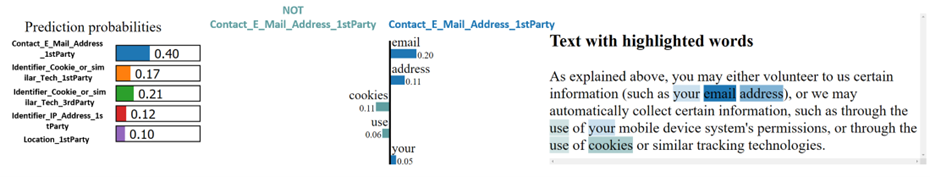
\includegraphics[width=1\linewidth]{figures/explanations_visualisations/counterfactual/3.3.png}
    \caption{Original explanation}
  \end{subfigure}
  \hfill
  \begin{subfigure}[b]{1\textwidth}
    \centering
    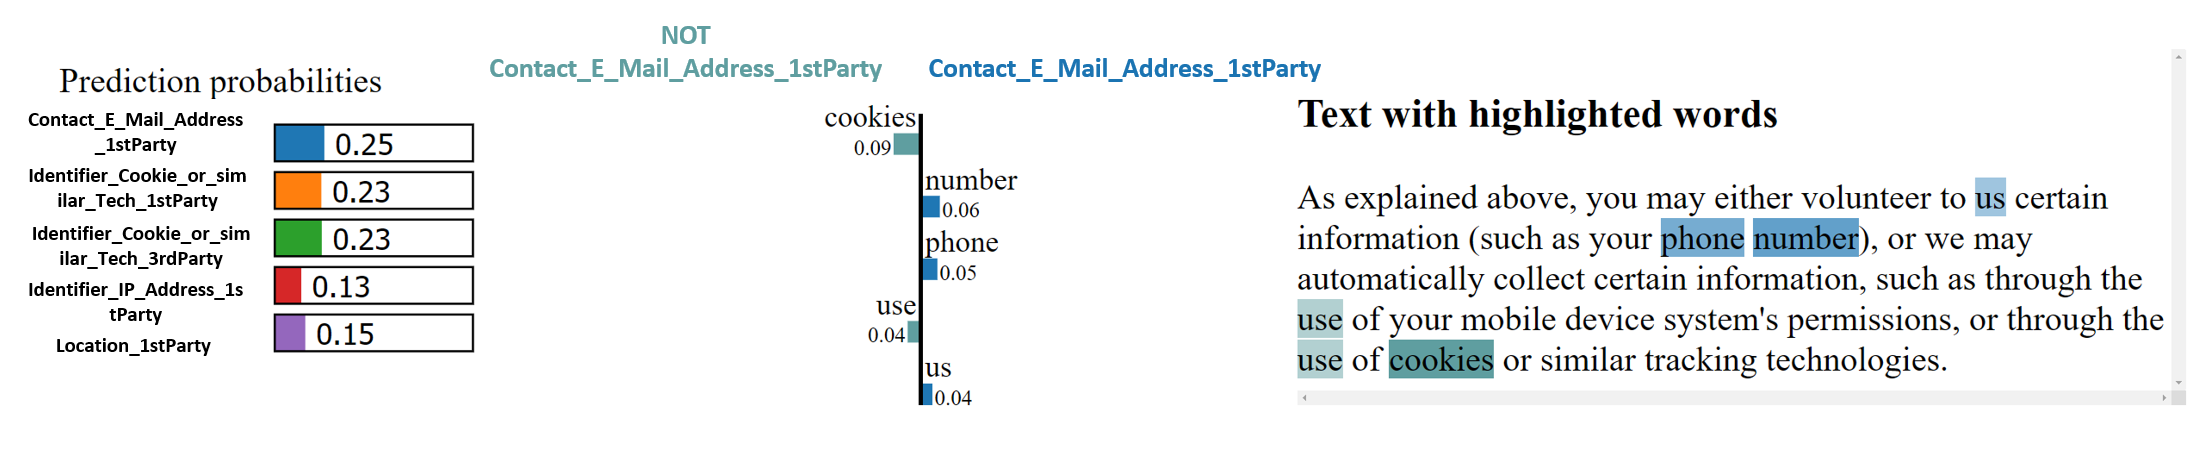
\includegraphics[width=1\linewidth]{figures/explanations_visualisations/counterfactual/3_3_counterfactual.png}
    \caption{Counterfactual explanation (not shown to respondents)}
    \label{fig:part3_counterfactual_1}
  \end{subfigure}
  \caption{Sample counterfactual explanation (1 out of 3)}
  \label{fig:part3_counterfactuals_example}
\end{figure}

\begin{figure}[!ht]
    \centering
    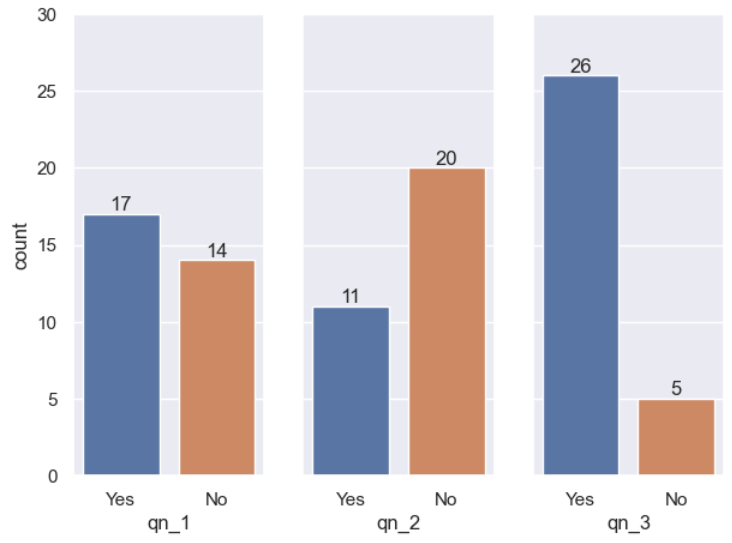
\includegraphics[width=1\linewidth]{figures/part_3_counterfactual.png}
    \caption{Votes for predicting whether counterfactual would be classified as \texttt{Identifier\_Cookie\_1st\_Party}}
    \label{fig:part3_counterfactual}
\end{figure}

\section{Part 4 \& 5: Testing which model and text representation is more understandable}
As there were three questions in each section to test the explainability of each pair of text representation and model, I totalled up the votes for each option for each part and each question (Figure~\ref{fig:part4} and~\ref{fig:part5}).

Overall, respondents found no difference in understandability between logistic regression and SVC (Figure~\ref{fig:part4}), while it was more contentious when comparing text representations, with a third split across the three options (Figure~\ref{fig:part5}). 

Remember that in terms of specific \hyperref[fig:heatmaps_perf]{class performance} of \texttt{Identifier Cookie 1st Party}, the performance difference between the classifiers that controlled for SVC but varied the text representation was higher than the difference for classifiers that controlled for GloVe but varied the model. Assuming that higher classifier performance correlates with higher understandability, when comparing respondents' votes with the "ground truth" metric of classifier performance, most respondents would be expected to indicate that there were differences in the understandability when comparing SVC + Tf-IDF vs SVC + GloVe, but no differences for SVC + GloVe vs logistic regression + GloVe. 

This second hypothesis is validated (Figure~\ref{fig:part4}) since the overwhelming majority of respondents chose "no difference". For the first hypothesis, while there were no majority votes for one option, votes were almost equally split instead of being heavily weighted in favour of one option (Figure~\ref{fig:part5}). This could suggest that respondents were more undecided about the understandability of the classifiers which somewhat reflects their similar performance figures. Overall, these results provide some support for some relation between understandability and classifier performance.

\begin{figure}[!ht]
  \centering
    \begin{subfigure}[b]{0.75\textwidth}
      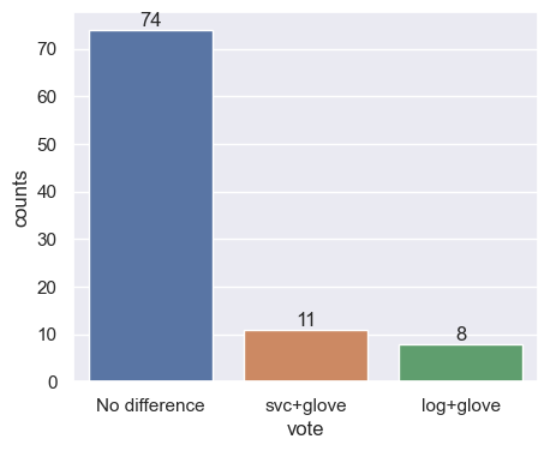
\includegraphics[width=1\linewidth]{figures/part4_votes.png}
      \caption{Total votes across 3 questions}
      %\label{fig:draketl}
    \end{subfigure}
    \hfill
    \centering
    \begin{subfigure}[b]{1\textwidth}
      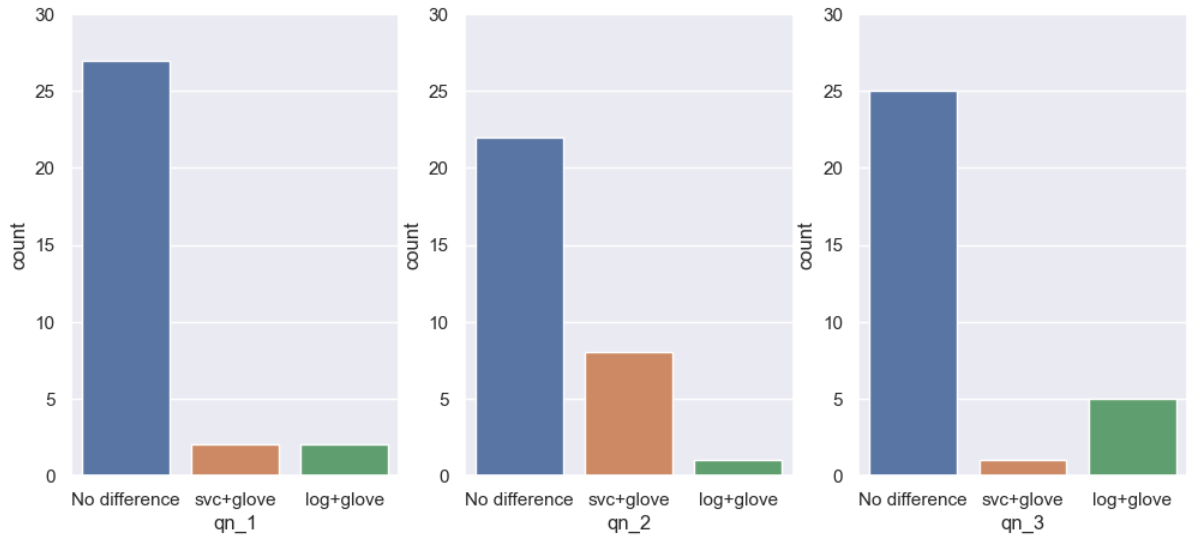
\includegraphics[width=1\linewidth]{figures/part_4_votes_1.png}
      \caption{Votes per question}
    \end{subfigure}
    \caption{Respondents' votes to whether SVC + GloVe (55\% F1) or Logistic regression + GloVe (59\% F1) were more understandable. F1 scores refer to specific class performance for \texttt{Identifier Cookie 1st Party}.}
    \label{fig:part4}
\end{figure}

\begin{figure}[!ht]
  \centering
    \begin{subfigure}[b]{0.75\textwidth}
      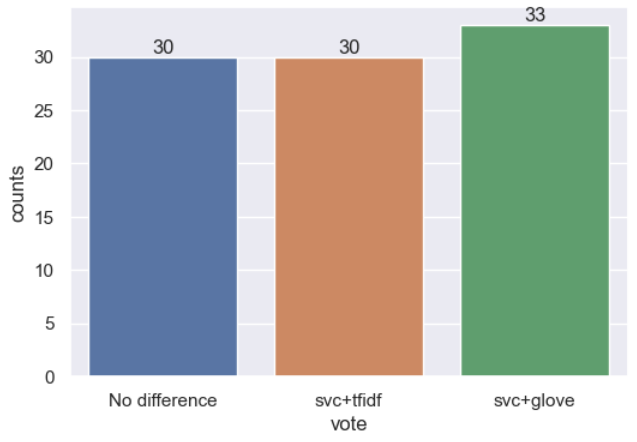
\includegraphics[width=1\linewidth]{figures/part5_votes.png}
      \caption{Total votes across 3 questions}
      %\label{fig:draketl}
    \end{subfigure}
    \hfill
    \centering
    \begin{subfigure}[b]{1\textwidth}
      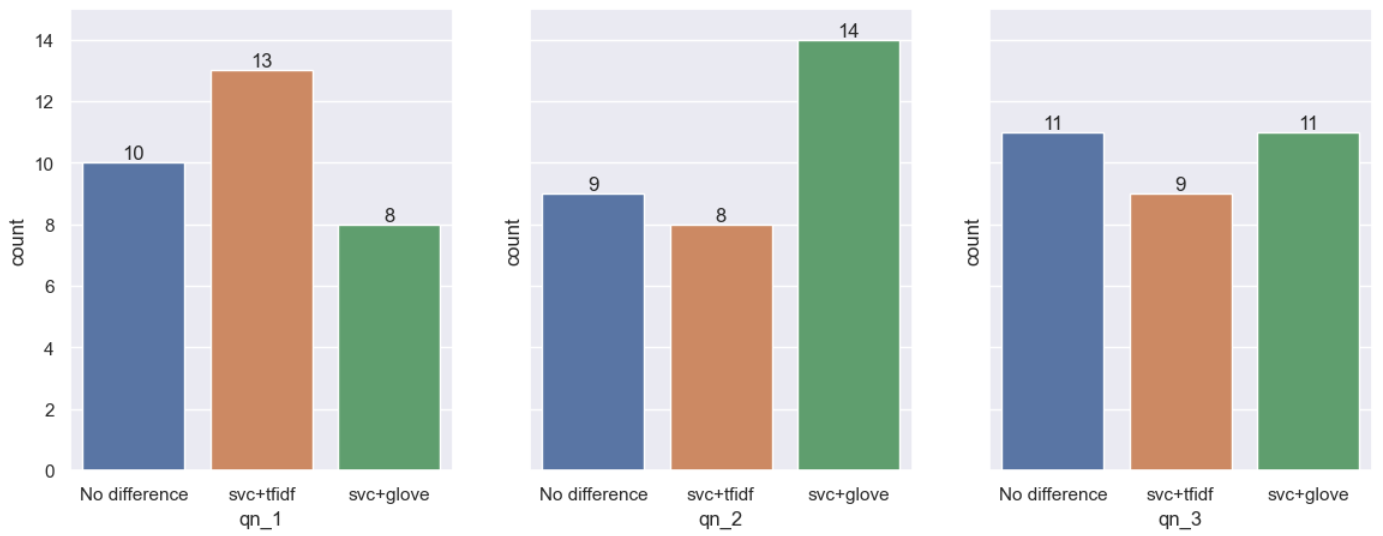
\includegraphics[width=1\linewidth]{figures/part_5_votes_1.png}
      \caption{Votes per question}
    \end{subfigure}
    \caption{Respondents' votes to whether SVC + Tf-IDF (68\% F1) or SVC + GloVe (55\% F1) were more understandable. F1 scores refer to specific class performance for \texttt{Identifier Cookie 1st Party}.}
    \label{fig:part5}
\end{figure}
